\subsection{Sicherheit und Datenschutz}

%Sicherheit und Datenschutz: Identifizieren Sie mögliche Sicherheitsrisiken und Datenschutzaspekte in der Unternehmenssoftware und zeigen Sie entsprechende Schutzmechanismen

Datensicherheit und Datenschutz sind gerade dann wenn, wie im Falle von PhileTipTip, personenbezogene Daten erhoben, verarbeitet und gespeichert werden von äußerster Wichtigkeit. Die Risiken, die mit diesen Themen verbunden sind, sollten daher noch einmal gesondert betrachtet werden und den jeweiligen Risikoeigentümern und Risikobearbeitern bewusst gemacht werden.\\

Betrachtet man die App gesondert von der Datenbank und dem Admin Tool kommt noch eine weitere Besonderheit hinzu - die Zugriffsrechte auf Systemfunktionen und Speicherstruktur des Smartphones des jeweiligen Nutzers. Da der Zugriff auf die GPS Koordinaten, die die Bestimmung des genauen Standorts erlauben und der Kamera sowie dem internen Speicher Rückschluss und Zugriff auf sensible Daten gestatten, ist es wichtig, diese Eingriffe so gering und für den Nutzer so nachvollziehbar wie möglich zu halten.\\

\begin{figure}[!h]
\centering
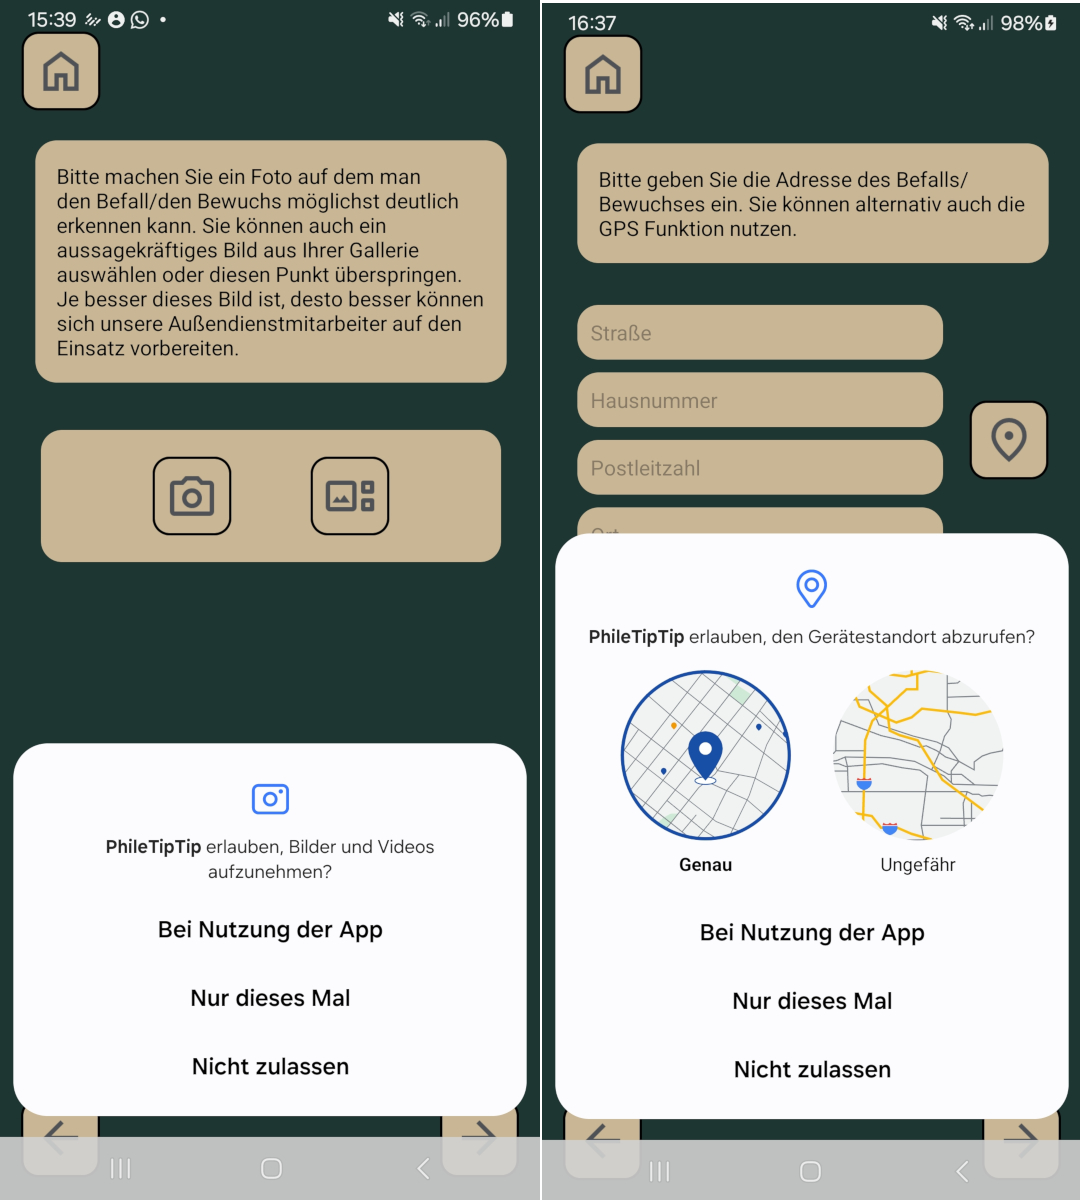
\includegraphics[width=0.6\textwidth]{Zugriffsrechte}
\caption{Zugriffsrechtabfrage - eigene Darstellung, Screenshot der PhileTipTip App}
\end{figure}

Die Abfrage an der Stelle, an der die Funktionalität benötigt wird und nicht gleich zum Aufstarten der App schafft Vertrauen beim Benutzer, da transparent wird, welche Funktion des Geräts für welchen Schritt in der Erfassung benötigt wird. Nach dem Grundsatz der Datensparsamkeit werden auch wirklich nur benötigte Funktionen abgefragt - das Popup, welches GPS Zugriff anfordert wird ein Nutzer nicht zu Gesicht bekommen, wenn er die Adresse selbst einträgt, ebenso wird ein Nutzer, der ein Bild aus seiner Gallerie läd nach Zugriff auf den Medienspeicher seines Smartphones gefragt, allerdings nicht nach dem Zugriff auf die Kamera.\\

\paragraph{Softwareseitige Risiken, die vom Entwicklerteam berücksichtigt und vermieden werden müssen sind unter anderem:}

\underline{SQL Injections}, die ein Risiko für die Integrität der Datenbank darstellen. Bei dieser Art des Angriffes wird über ein unzureichend abgesichertes Formularelement eine ausführbare MySql Anweisung übertragen, die dann auf dem Server interpretiert wird und dort entweder Zugangsüberprüfungen umgeht, Daten ausließt, manipuliert oder beschädigt. Diese Art des Angriffs ist weit verbreitet, aber auch gut zu verhindern, sofern sich die Entwickler dieser Gefahr bewusst sind \cite{sqlInjections}.

%https://www.invicti.com/blog/web-security/sql-injection-cheat-sheet/

\paragraph{Hardwareseitige Risiken, die von der IT-Abteilung berücksichtigt und vermieden werden müssen sind unter anderem:}

\underline{DDOS Angriffe}: Bei dieser Art des Angriffs wird der attackierte Server mit einer Vielzahl an Anfragen überlastet, bis seine Kapazitäten erreicht sind und er unerreichbar wird.\\
\underline{Serverausfälle}: Auch ohne externe Angriffe kann es zu Serverausfällen kommen, etwa durch Hardwareschäden oder Stromausfälle. Redundante Kopien (im Idealfall räumlich getrennt) und regelmäßige Backups begrenzen die Auswirkungen dieser Schäden und eine USV (Unabhängige Stromversorgung) stellt sicher, dass zumindest kurzfristige Stromausfälle überbrückt werden können.\\ Ein Offlinemodus der App, bei dem die Daten auf den lokalen Geräten vorgehalten werden, bis der Server wieder online ist ist ebenfalls eine Möglichkeit Datenverlust bei den Nutzern zu vermeiden, da diese die Erfassung der Schadstelle wie gewohnt durchführen können und das hochladen auf den Server verschoben wird, bis dieser wieder betriebsbereit ist.

\paragraph{Menschliche Risiken, die von den Anwendern berücksichtigt und vermieden werden müssen sind unter anderem:}

\underline{Social Engineering} ist eine Art des Angriffs, der weder auf Hard- noch auf Software, sondern auf den Mensch im System abzielt. Hierbei gibt sich der Angreifer zum Beispiel als Mitglied des IT-Supports aus und verlangt die Herausgabe des Passworts um so unberechtigt Zugriff auf die Daten zu erlangen. Um gegen diese Art des Angriffs geschützt zu sein ist es ratsam, ein gewisses Bewusstsein für Sicherheit bei den firmeninternen Nutzern zu schaffen, zum Beispiel durch Schulungen und klare Abläufe, wie der Support Kontakt zu den Mitarbeitern aufnimmt.\\

Bei den Nutzern außerhalb des Firmenökosystems (den Mietern und Eigentümern) sollte zumindest ein Hinweis eingeblendet werden, dass Phileteirus Immobilien GmbH niemals nach dem Passwort fragen wird um diese Gefahr zumindest abzumildern. Auch hier ist der Ansatz der Datensparsamkeit von hoher Wichtigkeit - da viele relevante Daten über Mieter, Mitarbeiter und Immobilieneigentümer bereits aus anderen Quellen vorliegen, können diese Nutzer sensibilisiert werden. Wenn sie es gewohnt sind, dass die App keinerlei Daten abfragt und anfordert, die nicht direkt mit dem Erfassungsprozess verbunden sind, werden sie im Falle eines Angriffs misstrauischer und vorsichtiger agieren und eventuelle Angriffe und Datenlecks schneller erkennen und melden.\\

\paragraph{Juristische Risiken, die von der Projektleitung und der Rechtsabteilung berücksichtigt und vermieden werden müssen sind unter anderem:}

\underline{Persönlichkeitsrechte - Recht am eigenen Bild}. Die PhileTipTip App erlaubt es den Nutzern Fotos von Schäden an Grünflächen anzufertigen um die Bewertung durch die Abteilung Außenabteilungen zu erleichtern. Daher ist es möglich, dass Personen auf den Bildern zu erkennen sind, die dem nicht zugestimmt haben. Hier muss auf eine juristisch haltbare Lösung hingearbeitet werden, etwa durch klar formulierte Allgemeine Nutzungsbedingungen der App, denen der Nutzer verbindlich zustimmt und somit selbst die Verantwortung übertragen bekommt die Privatsphäre Dritter zu wahren und zu achten.\\

Generell wird die Digitalisierung des Unternehmens, je weiter sie voranschreitet immer komplexer werden und die Berufung eines Datenschutzbeauftragten wird ab einem gewissen Punkt nicht nur sinnvoll, sondern notwendig werden um DSGVO (Datenschutzgrundverordnung) Konform zu handeln und somit rechtssicher auftreten zu können.